\documentclass{report}
\usepackage[utf8]{inputenc}
\usepackage[obeyspaces]{url}
\usepackage{mathtools}
\DeclarePairedDelimiter\ceil{\lceil}{\rceil}
\usepackage{amsmath}
\usepackage{amssymb}
\usepackage{natbib}
\bibliographystyle{plain}

\usepackage[all]{xy}
\usepackage{float}

\usepackage{amsthm}
\usepackage{todonotes}
\usepackage{array}
\usepackage{listings}
\usepackage{algorithm}
\usepackage{algorithmic}
\usepackage[a4paper]{geometry}


\makeatletter %otherwise geometry resets everything
\Gm@restore@org
\makeatother

\usepackage{hyphenat}

\newcommand{\GF}{\text{GF}}

\newcommand{\round}[1]{\mathrm{R_{#1}}}
\newcommand{\shift}[2]{{#1 \lll #2}}
\newcommand{\ThreeCircle}{{\sc ThreeCircle} }

\setlength{\itemsep}{0cm}
\setlength{\voffset}{0cm}
\setlength{\headheight}{0cm}
\setlength{\topmargin}{0cm}
\setlength{\extrarowheight}{3pt} %for superscripts in tabular
\setlength{\arraycolsep}{4pt}
\lstset{basicstyle = \footnotesize, breaklines = true}

\graphicspath{{imgs/}}

\begin{document}
\begin{titlepage}
\begin{center}
\textsc{\LARGE Research Internship\\Computer Science}\\[1.5cm]

\includegraphics[height=100pt]{imgs/logo}

\vspace{0.4cm}
\textsc{\Large Radboud University}\\[1cm]
\hrule
\vspace{0.4cm}
\textbf{\huge Report \& Documentation
}\\[0.4cm]
\hrule
\vspace{2cm}
\begin{minipage}[t]{0.45\textwidth}
\begin{flushleft} \large
\textit{Author:}\\
Tim van Dijk\\
\texttt{tim.vandijk96@gmail.com}
\end{flushleft}
\end{minipage}
\begin{minipage}[t]{0.45\textwidth}
\begin{flushright} \large
\textit{Internal supervisor/assessor:}\\
Prof. \, Joan Daemen\\
\texttt{j.daemen@cs.ru.nl}\\[1.3cm]
\texttt{}\\[1.3cm]
\textit{Second assessor:}\\
dr. \, Peter Schwabe\\
\texttt{peter@cryptojedi.org}
\end{flushright}
\end{minipage}
\vfill
{\large \today}
\end{center}
\end{titlepage}

\tableofcontents
\chapter*{Preface}
This document reports on the work I did during my research internship at the Digital Security Group at Radboud University. During the internship I was supervised by Joan Daemen, who let me work on topics that are related to his research.

Most students work on one project during the entirety of their research internship, but Joan and I chose to go with a different approach.
We instead chose to cover a wider range of topics, each for a couple of weeks, with the overarching theme being that it concerns cryptography over $\GF(p)$.

In Chapter 1, we work on implementing various field operations over $\GF(p)$ efficiently in ARM. In Chapter 2, we modify and implement the Walsh-Hadamard transformation Tto work in $\GF(p)$. In Chapter 3, we define the transformation \ThreeCircle and a scheme for computing MAC that works over $\GF(p)$. We then proceed to attack the scheme using differential cryptanalysis. Finally, in Chapter 4, we use the attack described in Chapter 3 to launch another attack that recovers the secret key used in the MAC scheme.

Relevant files are made available at:\\\url{https://github.com/TimVanDijk/Research-Internship-Public}.

\addcontentsline{toc}{chapter}{Preface}

\chapter{Efficient bitsliced implementations of field operations for ARM}

In this chapter, we will discuss the optimized bitsliced field operations that we implemented for ARM architectures. First we will provide some background information, after which we will discuss the implementations and possible improvements.

\section{Introduction}
Bitslicing is a term first coined Matthew Kwan in response to seeing Eli Biham present his paper \textit{A Fast New DES Implemenation in Software} in 1997.\cite{kwan1998bitslice}
Bitslicing refers to a software technique where a computation is expressed as a series of bitwise logical operations, such as AND, XOR, OR, NOT, NAND, NOR - as if you were implementing a logic circuit in hardware.
These computations are carried out in parallel, with as many simultaneous instances as there are bits in a register, performing the elementary operations on all bits of the register. The amount of parallelism is only bound by the target architecture's register width.

This technique can, for example, be used to efficiently implement certain ciphers. A requirement is that there is a high degree of parallelism on the operations that are performed on the state.
\newpage

In this document, we will show how bitslicing can be applied to emulate basic field operations, namely addition, multiplication and squaring, efficiently in $\GF(3)$, $\GF(5)$ and $\GF(7)$ using a regular binary computer.

In practice, in the foreseeable future, most data will continue to be represented in bits. Even if non-binary computers somehow take off, binary computers will still need to interface with them. These implementations can help binary computers to interface efficiently.

\subsection{Performing bitsliced computations}
To enable bitslicing, variables must be put in memory in a bit-sliced manner.
The straighforward way to store $n$ $m$-bit values, would to be to store each of the values in its own register (assuming at least $n$ registers with a width of at least $m$ bits are available).

A common method for putting values in a bit-sliced manner in memory is to transpose them. This means that we use $m$ registers of size $n$ (or larger) such that each register contains the bits of all $n$ values at one particular location. So if we let $r_{i,x}$ denote the $x$-th bit of register $r_i$, eventually the values are stored in memory in such way that $r_{i,x}$ equals the $i$-th bit of value number $x$.

Next, we need to reduce the computation we want to perform to a series of bitwise logical operations.
To this end, each bit in the output must be defined as a function of the input bits.
In most cases, it is trivial to find \emph{a} function that suffices: simply generate a truth table and extract an expression in the conjunctive normal form from it. 
However, this expression often is far from minimal, leading to a large amount of operations that must be applied to the data to get the desired result. Finding the function that uses the least amount of operations is key to creating the fastest possible implementation. Finding such a function often is quite challenging.

\subsection{Advantages of bitslicing}
There is a multitude of reasons as to why bitslicing can be advantageous.\cite{tabert2018bitslicing} A number of them are listed below:\\
\noindent\textbf{Speed.} In classical implementations, operations on specific bits of the state often require the relevant bits to be extracted first and permutations require a combination of shifts and masks.

In bitslicing, these operations can be performed much more efficiently as bits are readiliy available. Moreover, permutating bits does not require any operations at all, performing the permutation only mentally, given that it is kept in mind what represents what during subsequent computations.

Furthermore, as the code is extremely linear, it runs well on modern heavily pipelined CPUs as there is a low risk of branch misprediction, and there are plenty of opportunities for instruction reordering for efficient scheduling of data accesses.
\newpage
\noindent\textbf{Parallelization.} When the architecture has registers of width $w$ and the bitsliced operations take no longer than $w$ times as long, throughput increases. Of course, this is only applicable for workloads that allow for parallelization.\\
\noindent\textbf{Constant time.} Bitslicing is inherently protected against timing attacks.\\

\subsection{Disadvantages of bitslicing}
Bitslicing is not always the best solution nor can it always be used as a solution in the first place. Efficient bitslicing needs a huge amount of data-level parallelism, which simply is not always there. Furthermore, although throughput often increases, so does the delay. In some applications, this trade-off might be undesirable.

\subsection{ARM Cortex-M4}
We chose to develop the bitsliced implementations for the ARM Cortex-M4: a 32-bit microcontroller that has an ARMv7E-M architecture and it supports the ARMv7-M instruction set as well as the Thumb instruction set.\cite{cortexm4datasheet}

The device has 16 accessible registers: r0-r15. Of these, r0-r12 are general-purpose registers; r13 (sp) is the stack pointer; r14 (lr) is the link register and r15 (pc) is the program counter. All instructions can access r0-r14 and some can access r15 as well. In some cases, however, this leads to undefined behaviour which should be avoided.

On 32-bit ARM the calling convention is as follows:
\begin{itemize}
    \setlength\itemsep{0em}
    \item r0-r3 hold argument values passed to the subroutine. These values may be overwritten by the callee.
    \item r4-r11 are used to hold local variables. The callee must preserve the values in these registers.
    \item r12 is an ``Intra-Procedure-call scratch register'' whose content may be freely be destroyed.
    \item The return value is put in r0.
    \item The return address is stored in r14 (lr).
\end{itemize}

\section{Method}
In order to deal with digits in $\GF(p)$ on binary computers, we need to encode them in binary. 
To express a number in $\GF(p)$, ideally $\ceil*{\log_2 p}$ bits are required. We seize this opportunity and store the encoded digits in a bitsliced manner i.e.\ transposed: register $r_i$ contains at position $x$ the $i$-th bit of value number $x$.

Remember, to enable bitslicing, we must express the operations in terms of logical bitwise operations. The bitsliced representation helps doing this: we must define each output bit as a function of the input bits.

It is very difficult to find efficient functions by hand, so to automatically find a (somewhat) efficient function, we make use of logic synthesis tools. We opted to use Logic Friday since it is relatively well known and easily available to download.

\subsection{Development workflow}
Below is a description of the workflow that was used making the implementations.

\subsubsection*{Step 1: build a truth table}
For each operation that we want to implement, a truth table must be generated first. \path{Script/truth_table.py} contains the script that generates truth tables for addition, multiplication and squaring: the operations that we are interested in. It is currently set to generate tables for $\GF(3)$, $\GF(5)$ and $\GF(7)$, although that can easily be tweaked by changing a parameter. Most of the script has to do with formatting the output such that Logic Friday can use it. Furthermore, to improve legibility, we added plently of explanatory comments.

\subsubsection*{Step 2: generate a boolean expression, minimize it and perform logic synthesis}
Start Logic Friday and select \path{File->Import Truth Table} to import the truth table. Then, to perform logic synthesis, click \path{Operation->Map To Gates} and select 2-In NOR, XOR, AND and OR.
Normally, we would only select XOR, AND and OR, but we are required to select at least one of the universal gates (NOR and NAND). This is unfortunate because there is no direct equivalent instruction in ARM that simulates those gates. Experimentally, we found that selecting NOR yields the best results. 

Next the program asks for instruction on how to minimize the boolean expression. Select ``exact'' and ``minimize each output independently''. Experimentally, we found that these settings yield the best results. A gate diagram should now appear.

\subsubsection*{Step 3: write ARM assembly}
Transforming the gate diagram into ARM assembly is a long, tedious and boring \textit{yet} very simple process.\\
Once implemented the function will be called from a C wrapper as follows:
\begin{verbatim}
func(inputA, inputB, output);
\end{verbatim}
\newpage
As specified by the calling convention, the result will be that r0 contains a pointer to inputA, r1 contains one to inputB and r2 contains one to the output array.
At the very beginning of the function, we preverve the value registers whose value must be retained (as specified by the calling convention). We do so by pushing them to the stack:
\begin{verbatim}
PUSH {r4-r9}    ; Pushes r4 up to r9 to the stack
\end{verbatim}
After that is done, we load the inputs from memory into registers. $a_0$ and $a_1$ contain the low and high bits of inputA respectively. Same goes for $b_0$ and $b_1$ but with inputB. We do so using the following instructions:
\begin{verbatim}
LDR r3, [r0]         ; Loads a0 into r3
LDR r4, [r0, #4]     ; Loads a1 into r4 
LDR r5, [r1]         ; Loads b0 into r5
LDR r6, [r1, #4]     ; Loads b1 into r6
\end{verbatim}
Then, we implement the gates one by one. Luckily, the gates are numbered and if we stick to that ordering, we will not run into any dependency issues. 
AND, OR and XOR, gates translate directly into assembly instructions: AND, ORR and EOR respectively. To implement NOR gates, we need two: an ORR instruction followed by a negation which I chose to implement as an XOR with a value where all bits are set. For example, if we want to compute a0 NOR b1, we would do so as follows:
\begin{verbatim}
ORR r7, r3, r6           ; Compute a0 AND b1
EOR r7, r7, #0xffffffff  ; Negate the result
\end{verbatim}
At the end of the procedure we write the result to the output array:
\begin{verbatim}
STR r4, [r2]        ; Store c0 (in r4) to output[0]
STR r3, [r2, #4]    ; Store c1 (in r3) to output[1]
\end{verbatim}
Note that the offsets in the assembly are multiplied by 4. This is although the STR instruction stores a 4 byte value, it has a resolution of 1 byte.

Finally, we restore the preversed register values and jump to the return pointer, concluding the function:
\begin{verbatim}
POP {r4-r9}       ; Load r4 up to r9 from the stack
BX lr             ; Jump to return pointer
\end{verbatim}

\section{Results}
To measure the performance of the implementations, we counted the number of cycles a single execution takes on a STM32F407 Discovery board. All files can be found in \path{CycleCount/}.

In order to run the bitsliced operations on an actual device instead of a simulator, it had to be ported such that it could be compiled with the GNU Arm Embedded Toolchain. We failed to get accesses to memory to work, causing the result to be incorrect for addition in $\GF(7)$. Due to time constraints, we did not correct this mistake as it has no effect on the cycle count.

To compile the code, flash the device and perform the experiment, we used the following command:
\begin{verbatim}
make clean; make; st-flash write countcycles.bin 0x8000000
\end{verbatim}
Simultaneously, we would run \path{listener.py} to retrieve output over USART.

To gather results, each operation is run 25 times with pseudo-random input values. As expected the operations run in constant time and the results are summarized in Table \ref{fig:cnt}.
\begin{table}[ht]
\centering
\begin{tabular}{l|lll}
               & $\GF(3)$ & $\GF(5)$ & $\GF(7)$ \\ \hline
Addition       & 56    & 133   & 217   \\
Multiplication & 37    & 79    & 125   \\
Squaring       & 19    & 22    & 49   
\end{tabular}
\caption{Cycle count for the bitsliced operations.}
\label{fig:cnt}
\end{table}

\section{Discussion}
There still is a lot of room for improvement regarding the performance of the implementations - or to be more precise, the size of circuits that were implemented. Unfortunately, we only found after the research already was completed, that in 2009, Boothby and Brandshaw also looked into implementing various operations in $\GF(3)$, $\GF(5)$ and $\GF(7)$.~\cite{boothby2009bitslicing} Although they did not actually implement the operations they designed, it is clear that they would achieve much better performance. This mainly was due to two reasons:
\begin{enumerate}
\item An alternative representation for the numbers in the fields was used, allowing for more efficient boolean expressions to be generated;
\item The authors concluded that the Espresso heuristic (used by Logic Friday) performed very poorly, and resorted to a combination exhaustive search and manually puzzling instead.
\end{enumerate} 


\section{Future work}
One downside to using Logic Friday was that it can only output a diagram in image format. This adds an additional hurdle to automating the process of code generation, which made us choose to translate the diagrams into code manually.
If the diagram could be outputted in a more useful format, automatic code generation would have been very feasible and would most definitely be a better approach:
it would generate flawless implementations in one go and would save the developer hours of tedious menial work. Furthermore, the effort required to implementations manually increases dramatically as the size of the field increases. Considering the size of the operations in $\GF(7)$, We highly doubt implementing operations for $\GF(11)$ would be feasible. 

It also might be interesting to look into using SAT-based algorithms for logic minimization, as it is possible that they can be used to generate minimal expressions.
% ter info: Ko Stoffelen heeft dit gedaan

\chapter{The multi-dimsionsal discrete Fourier transform for $\GF(p)$}

The Walsh-Hadamard transform~\cite{wiki2018transform} is an important tool in linear cryptanalysis of mappings operating on vectors of elements of $\GF(2)$.
This chapter is about how we implemented the equivalent of the Walsh-Hadamard transform for mappings operating on vectors of elements of ${\GF(p)}$: the multi-dimensional discrete Fourier transform.

\section{Introduction}

Linear cryptanalysis exploits large correlations over all but a few rounds of a block cipher. The Walsh-Hadamard transform can be used to compute the correlation of a function with all linear functions, making it a very valuable tool.

We implemented the multidimensional discrete Fourier transform (MDFT) that this the equivalent for $\GF(p)$ of what the fast Walsh-Hadamard transform is for $\GF(2)$. While correlations in mappings over $\GF(2)$ are rational numbers, the correlations for mappings over $\GF(p)$ are complex numbers, with the real and imaginary part often non-rational. Indeed, correlations for such mappings have a magnitude and a phase. The complex nature of these correlations makes their interpretations non-trivial and a considerable part of our effort went into expressing correlations in such a way that they are easier to interpret.
\newpage
\noindent We did the following implementations:
\begin{enumerate}
\item MDFT for functions from ${\GF(p)}^n$ to ${\GF(p)}$, where correlations are coded as a couple of floating point numbers representing the real and imaginary part.
\item MDFT for functions from ${\GF(p)}^n$ to ${\GF(p)}$, where correlations are coded in full precision, with tuples of integers, and accompanying interpretation functions.
\item MDFT for mappings from ${\GF(p)}^n$ to ${\GF(p)}^m$, i.e., for mapping that have as output a tuple of multiple elements of $\GF(p)$, where correlations are coded in full precision.
\end{enumerate}

In the remainder of this chapter, we will discuss these variantions and their implementations.

\section{Method}
\subsection{MDFT for GP($p$)}
As we did not find a good description of the multidimensional discrete Fourier transform, we used as a starting point, the ``Python Example Code'' from the Wikipedia page on the Fast Walsh-Hadamard transform \cite{wiki2018transform}:
\begin{verbatim}
def fwht(a):
  h = 1
  while h < len(a):
    for i in range(0, len(a), h * 2):
       for j in range(i, i + h):
          x = a[j]
          y = a[j+h]
          a[j] = x + y
          a[j+h] = x - y
    h *= 2
\end{verbatim}

We then adjusted this code to also compute correlations over $\GF(p)$. In MDFT the $p$-th roots of unity in the complex plane take the place of $1$ and $-1$ in the Walsh-Hadamard transform. We denote the first root of unity as $\omega = e^{\frac{2\pi i}{p}}$.

\begin{verbatim}
def mdft(a, forward=True):
  w = omega() if forward else omega().conjugate()
  
  h = 1
  while h < len(a):
    for i in range(0, len(a), h * p):
      for j in range(i, i + h):
        temp = [a[j + k*h] for k in range(p)]

        for k in range(p):
          a[j + k*h] = sum([w**(k*l) * temp[l] for l in range(p)])

    h *= p
  return arr
\end{verbatim}
% JDA: naam van path misschien veranderen
This implementation can be found in \path{Hadamard/hadamard_transform.py}.

\subsection{MDFT for $\GF(p)$ with full precision}

For this implementation, instead of using floating point values, we used only exact values.
To do this, we needed an exact representation for the numbers we are working with.
The complex numbers we were using can be expressed as polynomials of the form:
\begin{equation*}
a_0\omega^0 + a_1\omega^1 + \dots + a_n\omega^n \quad with \quad \omega = e^{2\pi i/p} \text{ and } a_i = \frac{m}{p^j} \text{ with }  m, j \in \mathbb{N}
\end{equation*}
We can store such a polynomial using an array containing $a_0, \dots, a_n$. 
These polynomials were implemented as a class called ComplexPolynomial for which addition, multiplication, substraction, power and string functions were overloaded. This allowed the code that performs the MDFT with full precision to remain nearly unchanged. It can be found in \path{Hadamard/hadamard_transform_infinite_precision.py}\\

\subsubsection{The ComplexPolynomials class}
At the core of the program stand the complex polynomials, that are implemented in the ComplexPolynomials class which can be found at \path{Hadamard/ComplexPolynomial.py}. In addition to overloading several operations, this class contains the following utility functions:\\
\noindent\textbf{\textit{num}} returns a floating point approximation of the complex value of the polynomial.\\
\noindent\textbf{\textit{scaled}} returns a string representation of the current polynomial where each coefficient is divided by a given divisor.\\
\noindent\textbf{\textit{euler}} repeatedly applies Euler's formula which states that $e^{ix} = cos(x) + isin(x)$ to the polynomial, resulting in a string representation of the polynomial in terms of $cos$, $sin$, $\pi$, $p$ and $i$ where real and imaginary parts are clearly separated.\\
\noindent\textbf{\textit{phase}} returns a string representation of the exact phase. To be more precise, it first uses \textit{euler} to transform the polynomial into a real and an imaginy part. This is useful as we can see the imaginary part as the opposide side of the triangle and the real part as the adjacent side. Knowing this, we can express the phase as $tan^{-1}(opposide/adjacent)$.\\
\noindent\textbf{\textit{phase\_approx}} returns a floating-point value of the phase. It does this by calling \textit{num} and then using the phase function from the cmath library.\\
\noindent\textbf{\textit{polar\_approx}} returns a floating-point value of $r$ and $\theta$ that together constitute the polar coordinates of the polynomial. It achieves this by using other utility function to compute the required values.\\
\noindent\textbf{\textit{conjugate}} uses that the powers of $\omega$ are in modulus $p$.
This means that the inverse of $\omega^n$ is $\omega^{p-n}$ as $\omega^n * \omega^{p-n} = \omega^p = \omega^0 = 1$.
It returns the conjugate of the polynomial and does so simply by inverting the order of all but the first of the coefficients.\\
\noindent\textbf{\textit{magnitude}} uses \textit{euler} and the Pythagorean theorem to return a string representation of the exact magnitude of the polynomial.\\
\noindent\textbf{\textit{magnitude\_approx}} uses \textit{num} and the Pythagorean theorem to return a floating-point value of the magnitude.

\subsection{MDFT for mappings with multi-dimensional outputs}

This variant can be found in \path{Hadamard/hadamard_transform_alternative.py}.

\section{Results}
We added a number of variants of the Walsh-Hadamard transform the cryptanalysist's toolbox for systems that work over $\GF(p)$.

\section{Future work}
Currently, when a Complex Polynomial is displayed using the euler function, the result is very large (yet fully precise). One could try to simplify the resulting expression to make it more legible. Furthermore, if an operation is performed on a Complex Polynomial that could cause one of the terms to become a fraction, the result is not a Complex Polynomial, but a string. An enhancement could be to use fractions instead of integers to store $a_i$.

\chapter{Finding MAC collisions using differential cryptanalysis}
In this chapter, we describe how we apply differential cryptanalysis to find collisions in a MAC scheme that is based on (round-reduced) transformations. The transformation we use is the cryptographic transformation \ThreeCircle that operates over $\GF(3)$.

\section{Specification of \ThreeCircle}
\ThreeCircle is an experimental transformation for gaining insight in propagation.
It has a classical iterated structure: it iterates a round function a number of times to the state. This round function is designed according to the wide trail strategy: it contains a non-linear step, a mixing step, two transposition steps and the addition of a (round-index-dependent) round constant. 

A \ThreeCircle state $a$ consists of $5$ $32$-digit lanes, we write $a = (a_0,a_1,a_2,a_3,a_4)$. 

\noindent
We list our notational conventions in Table~\ref{t:conventions}.

\begin{table}
\caption{\label{t:conventions}Notational conventions}
\begin{center}
\begin{tabular}{ll}\hline
$a_y$               & Lane $y$ of state $a$ \\
$a_{y,x}$           & Bit $x$ of lane $a_z$ \\
$\shift{a_y}{v}$    & Cyclic shift of $a_y$ moving digit in position $x$ to position $x+v$\\
$a_y + a_{y'}$      & Digitwise sum of lanes $a_y$ and $a_{y'}$ \\
$a_y a_{y'}$        & Digitwise product of lanes $a_y$ and $a_{y'}$ \\
\hline
\end{tabular}
\end{center}
\end{table}

The permutation consists of 12 rounds $\round{i}$ as specified in Algorithm~\ref{a:permutation}. 

\begin{algorithm}
\begin{algorithmic}
\FOR {Round index $i$ from $-11$ to $0$}
    \STATE $a \gets \round{i}(a)$
\ENDFOR
\STATE Here $\round{i}$ is specified by the following sequence of steps: 
\end{algorithmic}
\begin{displaymath}
\begin{array}{lll}
\chi:    & b_y & \gets a_y + \shift{a_{y+1}a_{y+1}}{1} \text{ for all } y \\
         & a   & \gets b\\
\theta:  & p   & \gets a_0 + a_1 + a_2 + a_3 + a_4\\ 
         & e   & \gets \shift{p}{12} + \shift{p}{17}\\
         & a_y & \gets a_y + e \text{ for all } y\\
\pi:     & b_y & \gets a_{y+1} \text{ for all } y\\
         & a   & \gets b\\
\iota    & a_0 & \gets a_0 + c_j \\
\rho:    & a_i & \gets \shift{a_y}{r_y} \text{ for all } y \text{ with } r = (0,2,6,11,19)\\
\end{array}
\end{displaymath}
\caption{\label{a:permutation} The \ThreeCircle round function $\round{i}$}
\end{algorithm}

The round constants $c_j$ are 32-digit lanes and as they are unimportant for the purpose of our research,
we specify them currently as all-zero.


\section{Computing MACs}
The scheme we use for computing MACs is illustrated in Figure \ref{fig:mac} and resembles the CBC-MAC scheme. To apply the scheme, we need a message $M$, segmented into parts $M_0, \dots, M_t$, a key $K$ and a round-based transformation $F$.

The first part of the message is added to the key and is then put through $n$-rounds of the transformation. The output then is added to the second part of the message and then again is put through the round-reduced transformation. This process is repeated until the last segment of the message is added. Then, $m$-rounds of the transformation with $m \gg n$ are applied. Finally, the key is added, resulting in the MAC.

\begin{figure}[!ht]
\centering
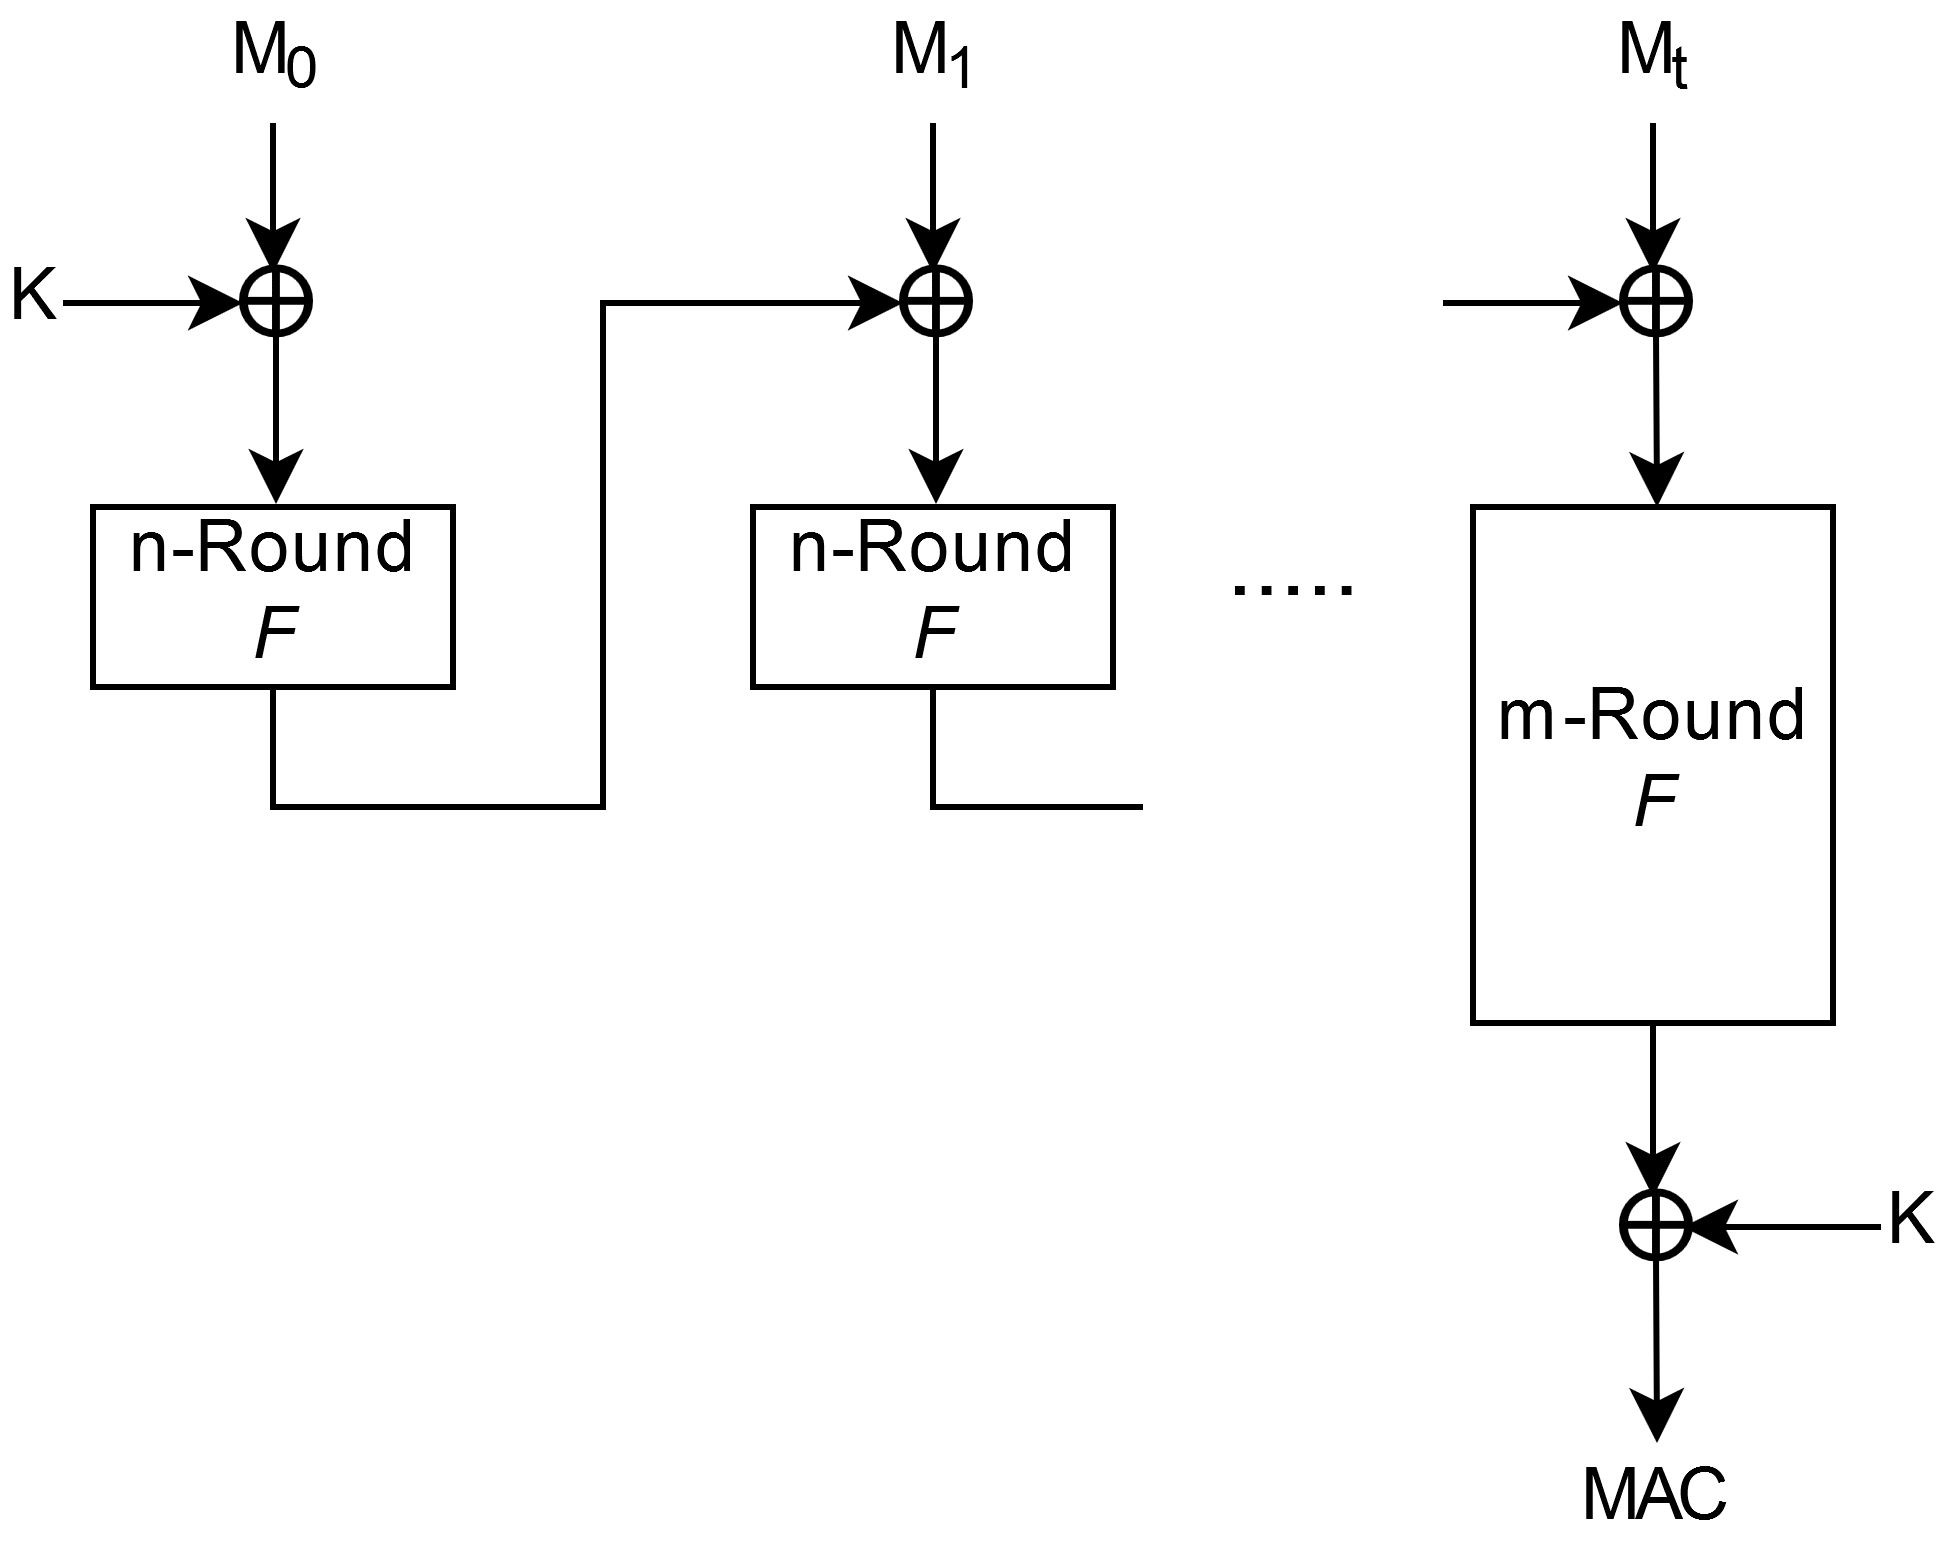
\includegraphics[scale=0.120]{imgs/HMAC_HighResV2.png}
\caption{Scheme for generating MACs using a (round-reduced) transformation.}
\label{fig:mac}
\end{figure}

In the MAC generation scheme, we use 3-round \ThreeCircle as the round-reduced transformation and use 12-round \ThreeCircle at the end i.e. $F$ = \ThreeCircle, $n=3$ and $m=12$. The resulting scheme is displayed in Figure \ref{fig:mac3c}.

\begin{figure}[!ht]
\centering
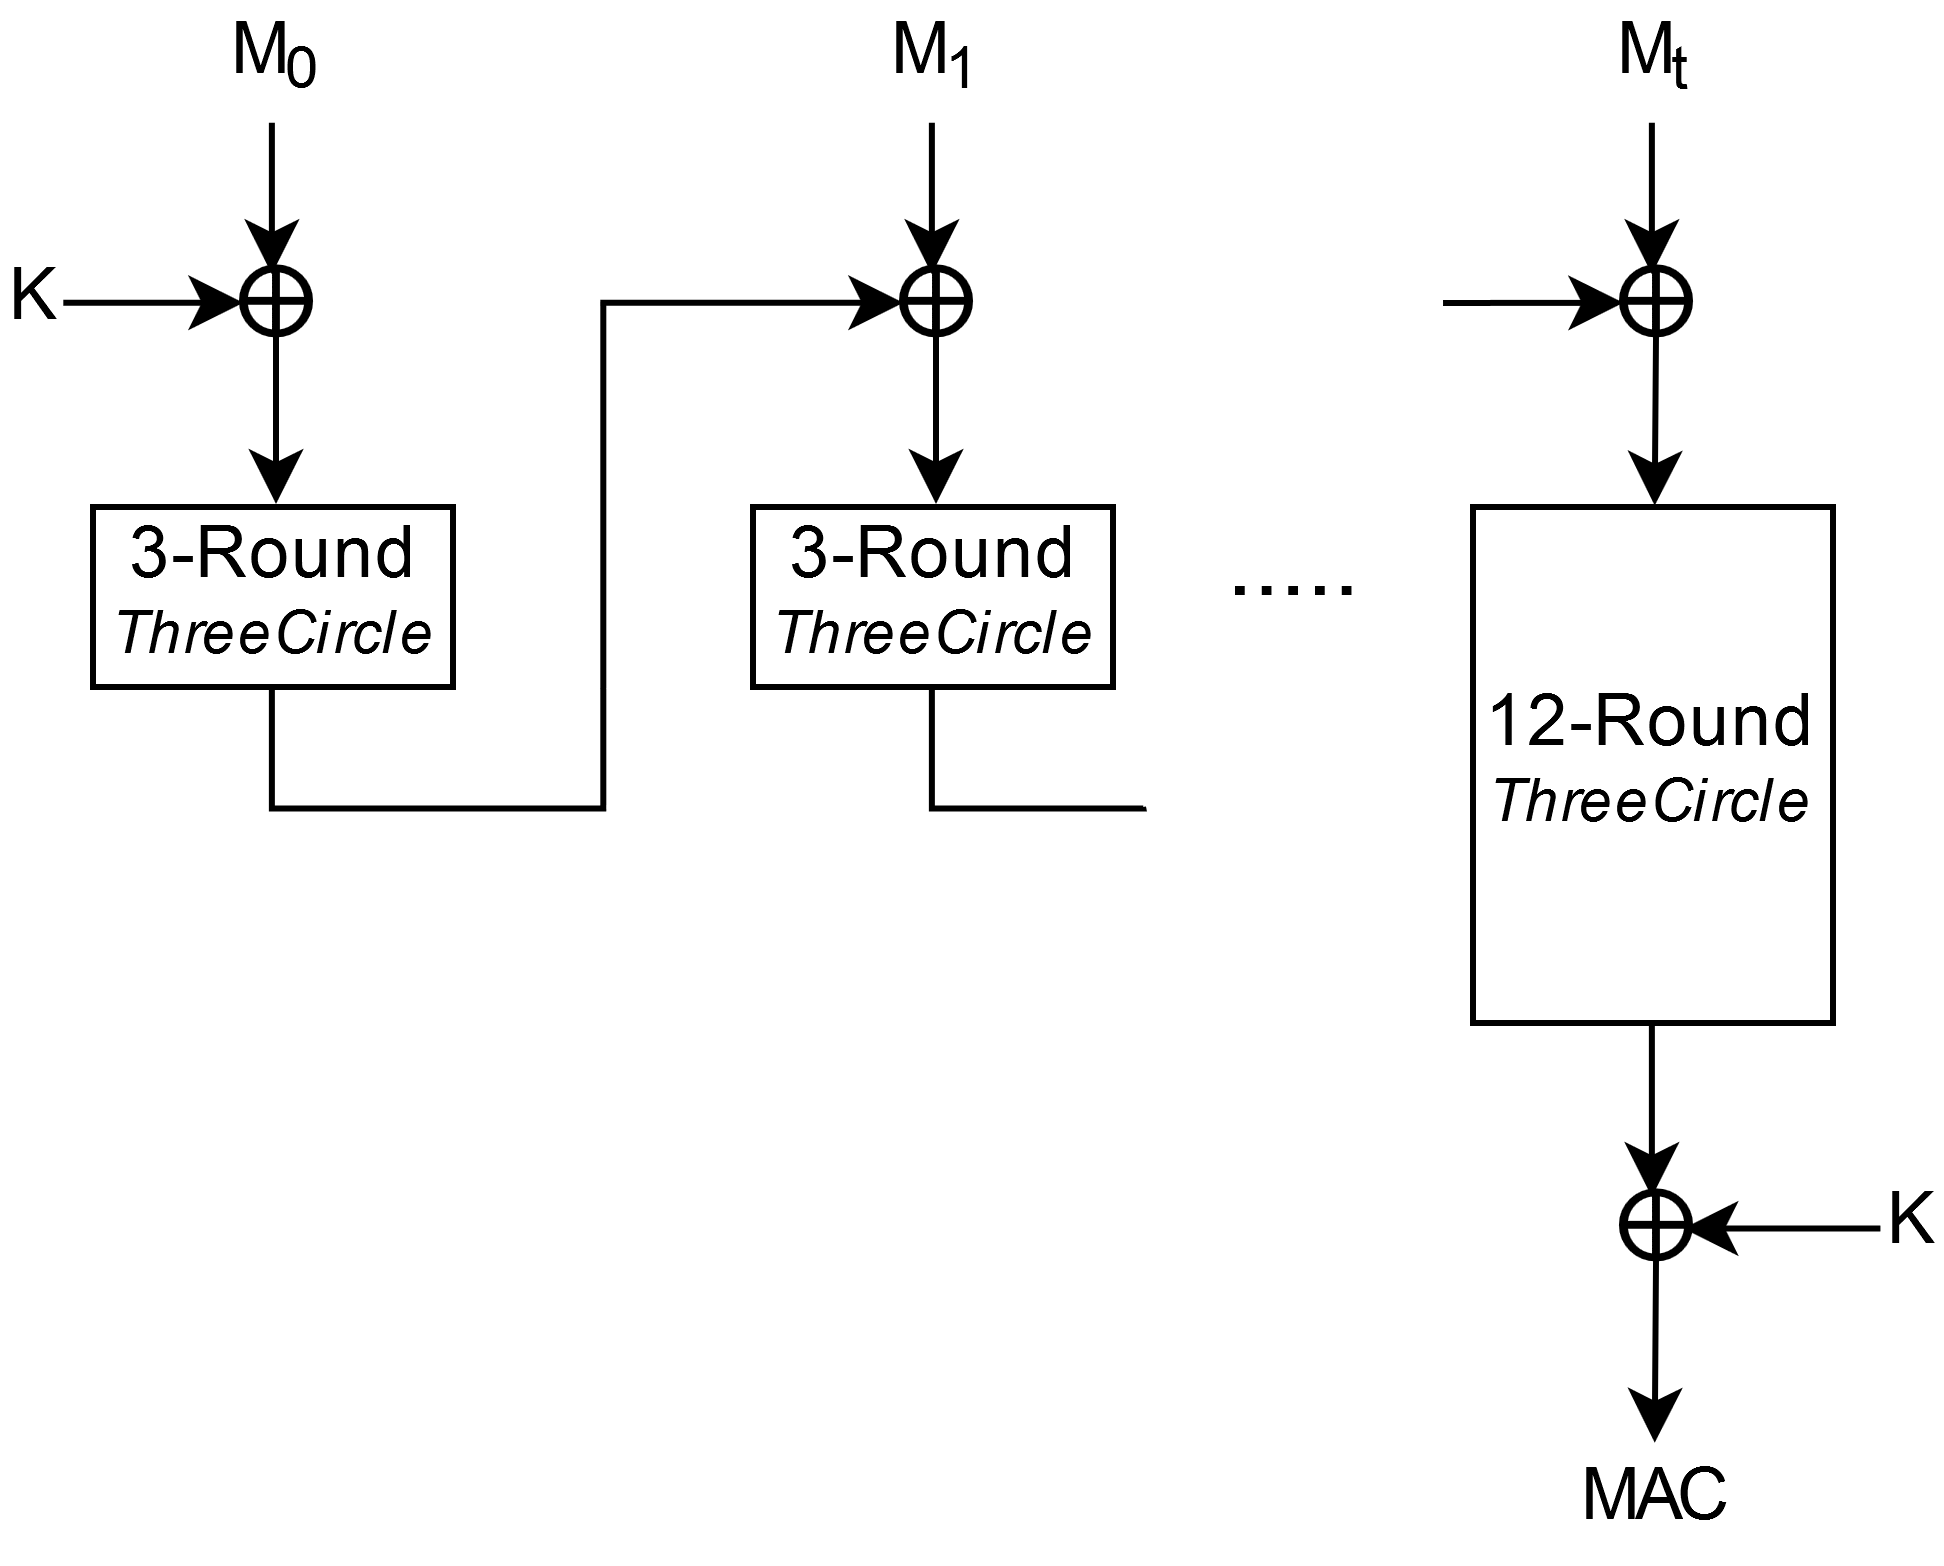
\includegraphics[scale=0.120]{imgs/HMAC_HighRes_ThreeCircle.png}
\caption{Scheme for generating MACs using (round-reduced) \ThreeCircle.}
\label{fig:mac3c}
\end{figure}

Since we designed \ThreeCircle, there was no implementation available yet. Therefore, we made one. It can be found in \path{DC/ThreeCircle.py}.

The implementation is made in Python and serves as a reference implementation that is to be used during our research. Consequently, there was no focus at all on optimization. The state is stored as a 2D list of integers. Since all digits are in $\GF(3)$, one could substantially optimize for memory by using only 2 bits to represent each digit. This representation allows for the use of the bitsliced implementations of field operations we made for ARM.

Implementing the transposition layer and its inverse was very straightforward, but the non-linear layer and mixing layer were not quite so. For that reason, we will elaborate on the implementations of those two layers.
\subsection{Implementing the non-linear layer}
The non-linear layer, $\chi$, is based on a simple non-linear function: $b_i = a_i + a_{i+1}^2$.
In the specification, $\chi$ is defined as:
\begin{equation*}
\begin{split}
b_y \leftarrow& a_y + a_{y+1}a_{y+1} \lll 1 \text{ for all } y\\
a \leftarrow& b
\end{split}
\end{equation*}
As you can see, the function is applied to an entire lane at once: lane $y$ gets replaced by the sum of lane $y$ and the shifted digit-wise square of lane $y+1$. On a digit level, it comes down to adding the square of the bottom-right neighbor to each digit. Note that \ThreeCircle $\chi$ has a single circle: if we start at any given digit in the state, and then repeatedly visit the bottom-right neighbor, we cover the entire state and eventually end up at the digit we started at.

\ThreeCircle $\chi$ is almost a bijection as only $2^{160}$ out of $3^{160}$ input values collide: $\frac{2^{160}}{3^{160}} = (\frac{2}{3})^{160} \approx 6.6895*10^{-29}$. This means that not all states have a preimage. To find an inverse, we guess the last digit of the state. This allows us to fill out the rest of the state as we can rewrite the function as $a_i \leftarrow b_i - a_{i+1}^2$.
In the end, we check if the equation also holds for the computed first digit and the (guessed) last digit. If we find a contradiction, the guess was wrong, so we try again with another guess. If the equation holds, the guess was correct and we have found a valid inverse.

\subsection{Implementing the mixing layer}
At first, this layer was defined as:
\begin{equation}
\begin{split}
&p \leftarrow a_0 + a_1 + a_2 + a_3 + a_4 \\
&e \leftarrow p \lll 12 + p \lll 17 \\
&a_y \leftarrow a_y + e \text{ for all } y
\end{split}
\tag{$\theta$}
\end{equation}
This is a column-parity mixer (CPM), but it had to be modified because it caused in weakness in combination with the simple non-linear layer. To correct this weakness, we introduced a shift:
\begin{equation}
\begin{split}
&p \leftarrow a_0 + a_1 + a_2 + a_3 + a_4 \\
&e \leftarrow p \lll 12 + p \lll 17 \\
&a_y \leftarrow a_y + (e \lll y) \text{ for all } y
\end{split}
\tag{$\theta$}
\end{equation}
Either way, implementing it was simple. The inverse, however, was more challenging.

This layer can be expressed as the multiplication of the parity with a matrix, namely the one generated by the following python code:
\begin{verbatim}
[[1 if j == (i+12) % 32 or j == (i+17) % 32 else 0 \
    for j in range(32)] for i in range(32)]
\end{verbatim}
In terms of CPM's, this matrix is called Z. However, since we are working in $\GF(3)$, and parities are not longer either even or odd, we were not done yet and had to rewrite some equations. As it turns out, we need to use Y instead of Z with $Y = 2*Z + I$. As the transformation now essentially is a matrix multiplication, we can invert the transformation by multiplying with the inverse of the matrix. To compute the inverse of the matrix, we used sage:
\begin{verbatim}
sage: import numpy as np
sage: Z = np.matrix([[1 if j == (i+12) % 32 or j == (i+17) % 32 \
    else 0 for j in range(32)] for i in range(32)])
sage: Y = 2*Z + np.identity(32)
sage: inv = Matrix(IntegerModRing(3), Y).inverse()
sage: print(inv)
[1 1 2 0 0 1 2 1 1 1 2 1 2 2 0 2 0 2 0 0 1 1 0 0 0 0 1 1 1 1 2 0]
[0 1 1 2 0 0 1 2 1 1 1 2 1 2 2 0 2 0 2 0 0 1 1 0 0 0 0 1 1 1 1 2]
[2 0 1 1 2 0 0 1 2 1 1 1 2 1 2 2 0 2 0 2 0 0 1 1 0 0 0 0 1 1 1 1]
[1 2 0 1 1 2 0 0 1 2 1 1 1 2 1 2 2 0 2 0 2 0 0 1 1 0 0 0 0 1 1 1]
[1 1 2 0 1 1 2 0 0 1 2 1 1 1 2 1 2 2 0 2 0 2 0 0 1 1 0 0 0 0 1 1]
[1 1 1 2 0 1 1 2 0 0 1 2 1 1 1 2 1 2 2 0 2 0 2 0 0 1 1 0 0 0 0 1]
[1 1 1 1 2 0 1 1 2 0 0 1 2 1 1 1 2 1 2 2 0 2 0 2 0 0 1 1 0 0 0 0]
[0 1 1 1 1 2 0 1 1 2 0 0 1 2 1 1 1 2 1 2 2 0 2 0 2 0 0 1 1 0 0 0]
[0 0 1 1 1 1 2 0 1 1 2 0 0 1 2 1 1 1 2 1 2 2 0 2 0 2 0 0 1 1 0 0]
[0 0 0 1 1 1 1 2 0 1 1 2 0 0 1 2 1 1 1 2 1 2 2 0 2 0 2 0 0 1 1 0]
[0 0 0 0 1 1 1 1 2 0 1 1 2 0 0 1 2 1 1 1 2 1 2 2 0 2 0 2 0 0 1 1]
[1 0 0 0 0 1 1 1 1 2 0 1 1 2 0 0 1 2 1 1 1 2 1 2 2 0 2 0 2 0 0 1]
[1 1 0 0 0 0 1 1 1 1 2 0 1 1 2 0 0 1 2 1 1 1 2 1 2 2 0 2 0 2 0 0]
[0 1 1 0 0 0 0 1 1 1 1 2 0 1 1 2 0 0 1 2 1 1 1 2 1 2 2 0 2 0 2 0]
[0 0 1 1 0 0 0 0 1 1 1 1 2 0 1 1 2 0 0 1 2 1 1 1 2 1 2 2 0 2 0 2]
[2 0 0 1 1 0 0 0 0 1 1 1 1 2 0 1 1 2 0 0 1 2 1 1 1 2 1 2 2 0 2 0]
[0 2 0 0 1 1 0 0 0 0 1 1 1 1 2 0 1 1 2 0 0 1 2 1 1 1 2 1 2 2 0 2]
[2 0 2 0 0 1 1 0 0 0 0 1 1 1 1 2 0 1 1 2 0 0 1 2 1 1 1 2 1 2 2 0]
[0 2 0 2 0 0 1 1 0 0 0 0 1 1 1 1 2 0 1 1 2 0 0 1 2 1 1 1 2 1 2 2]
[2 0 2 0 2 0 0 1 1 0 0 0 0 1 1 1 1 2 0 1 1 2 0 0 1 2 1 1 1 2 1 2]
[2 2 0 2 0 2 0 0 1 1 0 0 0 0 1 1 1 1 2 0 1 1 2 0 0 1 2 1 1 1 2 1]
[1 2 2 0 2 0 2 0 0 1 1 0 0 0 0 1 1 1 1 2 0 1 1 2 0 0 1 2 1 1 1 2]
[2 1 2 2 0 2 0 2 0 0 1 1 0 0 0 0 1 1 1 1 2 0 1 1 2 0 0 1 2 1 1 1]
[1 2 1 2 2 0 2 0 2 0 0 1 1 0 0 0 0 1 1 1 1 2 0 1 1 2 0 0 1 2 1 1]
[1 1 2 1 2 2 0 2 0 2 0 0 1 1 0 0 0 0 1 1 1 1 2 0 1 1 2 0 0 1 2 1]
[1 1 1 2 1 2 2 0 2 0 2 0 0 1 1 0 0 0 0 1 1 1 1 2 0 1 1 2 0 0 1 2]
[2 1 1 1 2 1 2 2 0 2 0 2 0 0 1 1 0 0 0 0 1 1 1 1 2 0 1 1 2 0 0 1]
[1 2 1 1 1 2 1 2 2 0 2 0 2 0 0 1 1 0 0 0 0 1 1 1 1 2 0 1 1 2 0 0]
[0 1 2 1 1 1 2 1 2 2 0 2 0 2 0 0 1 1 0 0 0 0 1 1 1 1 2 0 1 1 2 0]
[0 0 1 2 1 1 1 2 1 2 2 0 2 0 2 0 0 1 1 0 0 0 0 1 1 1 1 2 0 1 1 2]
[2 0 0 1 2 1 1 1 2 1 2 2 0 2 0 2 0 0 1 1 0 0 0 0 1 1 1 1 2 0 1 1]
[1 2 0 0 1 2 1 1 1 2 1 2 2 0 2 0 2 0 0 1 1 0 0 0 0 1 1 1 1 2 0 1]
\end{verbatim}
\newpage
Unfortunately, there is no ``clever'' approach to generating an inverse for $\theta$. We decided to go with the general approach.
Since $\theta$ is linear, we can find the inverse by applying it to each row of a 160x160 identity matrix and then computing the inverse of the result.
Again, we used sage to do this:
\begin{verbatim}
import numpy as np

from ThreeCircle import theta
from Util import *

inp = np.identity(160)
out = np.apply_along_axis(lambda x: from_state(theta(to_state(x))), \
    axis=1, arr=inp)

inv = Matrix(IntegerModRing(3), out).inverse()
\end{verbatim}
The result is a 160x160 matrix which is serialized and stored in \path{DC/theta_inv_matrix.dat}. We modified \ThreeCircle such that the inverse is a matrix multiplication of the state with our newly made matrix.

\section{Differential Cryptanalysis}
Differential Cryptanalsysis is the study of how differences in information input can affect differences in information output. In this chapter, we will use it to find MAC collisions. To this end, we need a trail or differential. Trails are knowledge of how an input difference propagates through the rounds and the probability of it happening. Differentials are very similar to trails, but here only the difference at the input and output is important and it does not matter how the difference propagates inbetween rounds.

As an example of what a differential is, consider the example in figure \ref{fig:diff}:
we start with two arbitrary messages $M_0$ and $M_1$ with a fixed difference, $\Delta_{in}$. Note that if we add the same value to both messages, the difference remains the same, so we have: 
\begin{equation*}
\Delta_{in} = M_1 - M_0 = (M_1 + K) - (M_0 + K)
\end{equation*}

Now, assume we have the following differential $(\Delta_{in}, \Delta_{out})$ for transformation $F$ with associated differential probability $DP(\Delta_{in}, \Delta_{out}) = p$. It means that with probability $p$, we have that:
\begin{equation*}
\begin{split}
\Delta_{out} &= F(M_1 + K) - F(M_0 + K) \\
&= (F(M_1 + K) + K) - (F(M_0 + K) + K) \\
&= Out_1 - Out_0
\end{split}
\end{equation*}

\begin{figure}[!ht]
\centering
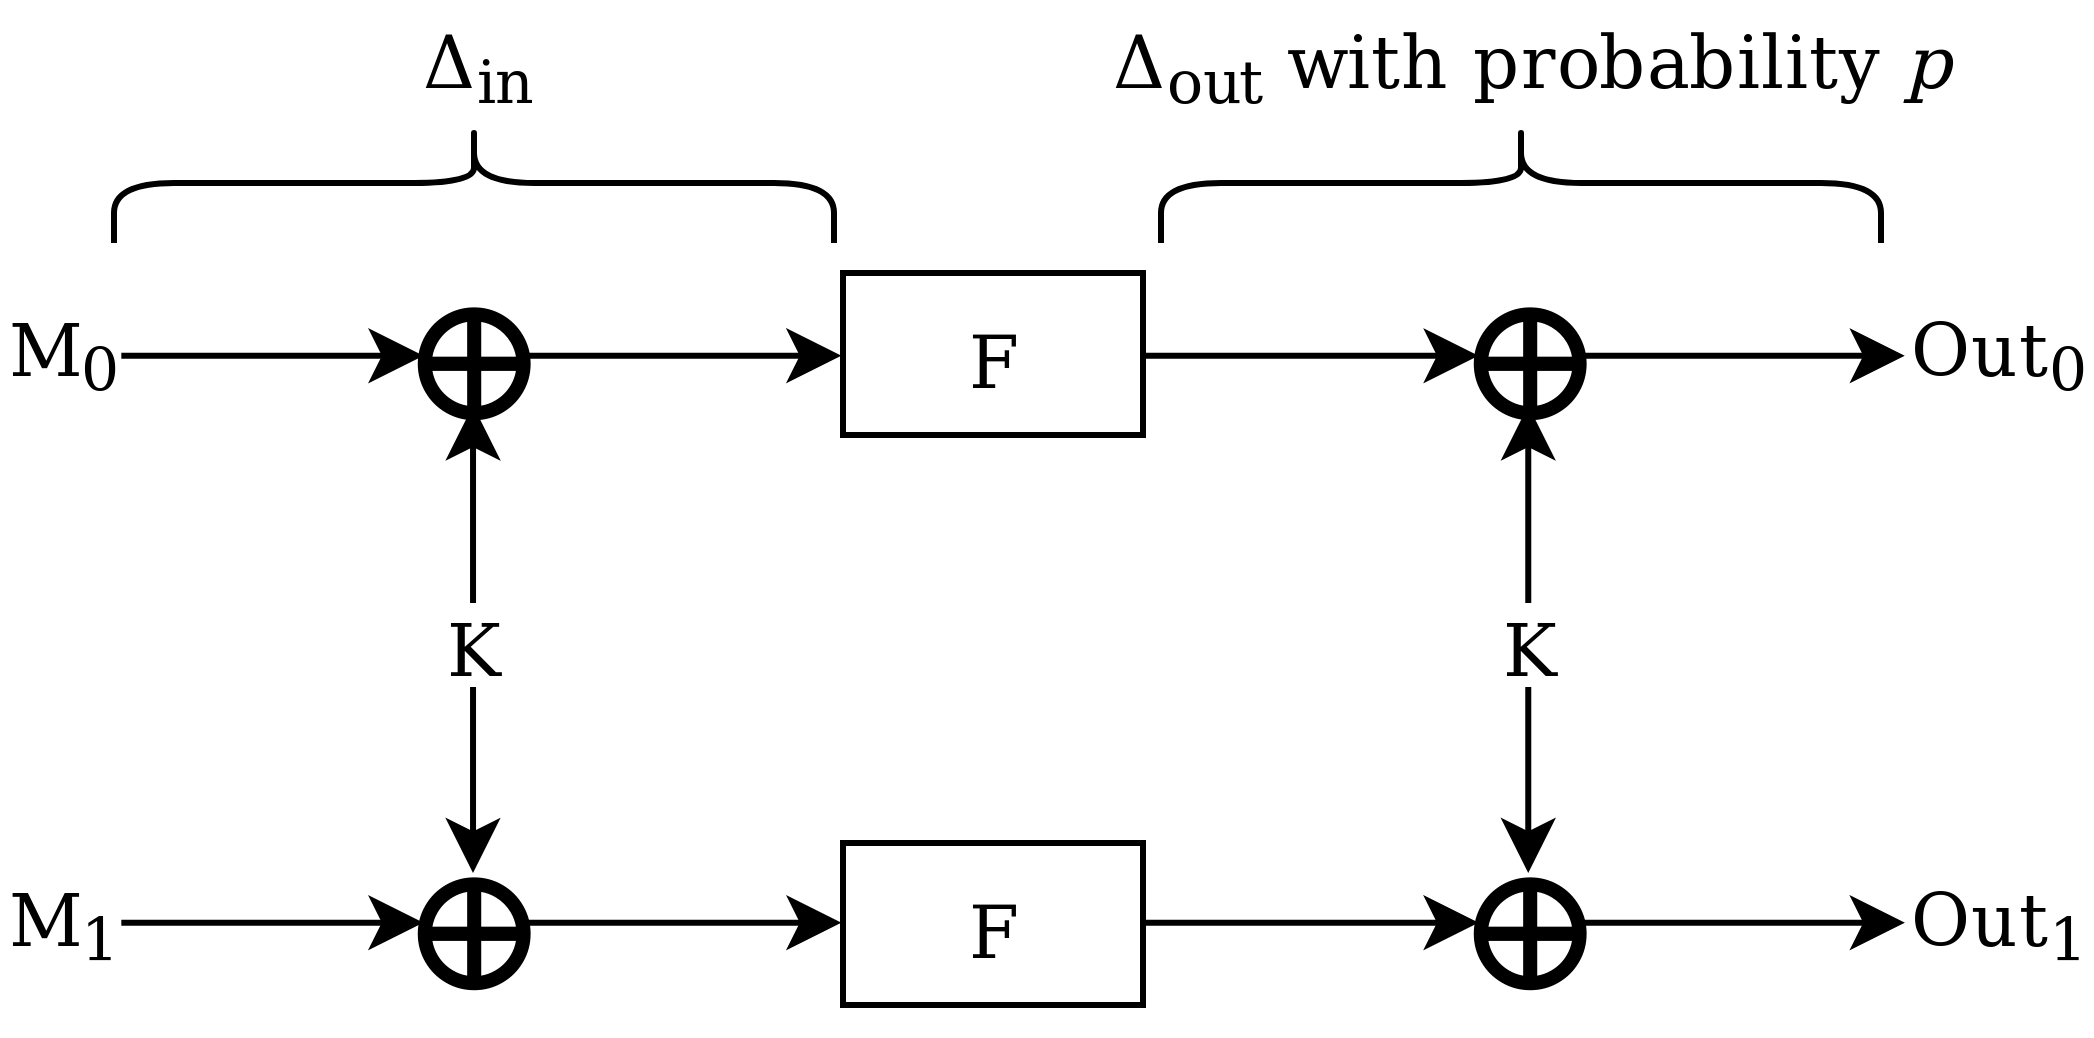
\includegraphics[scale=0.125]{imgs/Differential_Example.png}
\caption{Illustrated example of a differential.}
\label{fig:diff}
\end{figure}

\section{Finding collisions}
As it turns out, we can use differentials to find colliding MACs in the scheme using round-reduced transformations. How this can be achieved is shown in Figure \ref{fig:coll}.

We try to find two different messages $(A_0 || A_1)$ and $(B_0 || B_1)$ that have the same MAC. To understand why this technique for finding collisions works, we need to reason backwards a little.

In the end, the MACs are the same, so the difference is 0. This means that the values after 12-round \ThreeCircle also must be the same, since adding the same value to both does not affect the difference. 12 rounds of \ThreeCircle completely scrambles the input, and we can no longer say anything meaningful about the relation between input difference and output difference. The only way we can make the output values the same is by making sure the input values are the same. We will use the differential $(\Delta_{in}, \Delta_{out})$ to try and make this the case.

To use the differential, the input difference must equal $\Delta_{in}$. We can do so by randomly picking $A_0$ and setting $B_0 = A_0 + \Delta_{in}$. The key is added to both messages and 3 rounds of \ThreeCircle is applied to each. Our differential says that with probability $DP(\Delta_{in}, \Delta_{out})$, the values now have difference $\Delta_{out}$. We assume that this indeed is the case. In practise, the attack on average must be repeated $\frac{1}{DP(\Delta_{in}, \Delta_{out})}$ times for this to work.

Since we are free to choose the value of $B_1$, we can use it to compensate for the difference of $\Delta_{out}$. We can do so by setting $B_1 = A_1 - \Delta_{out}$. 
The addition now cancels out the difference, causing a difference of 0, meaning the values are the same.

\begin{figure}
\centering
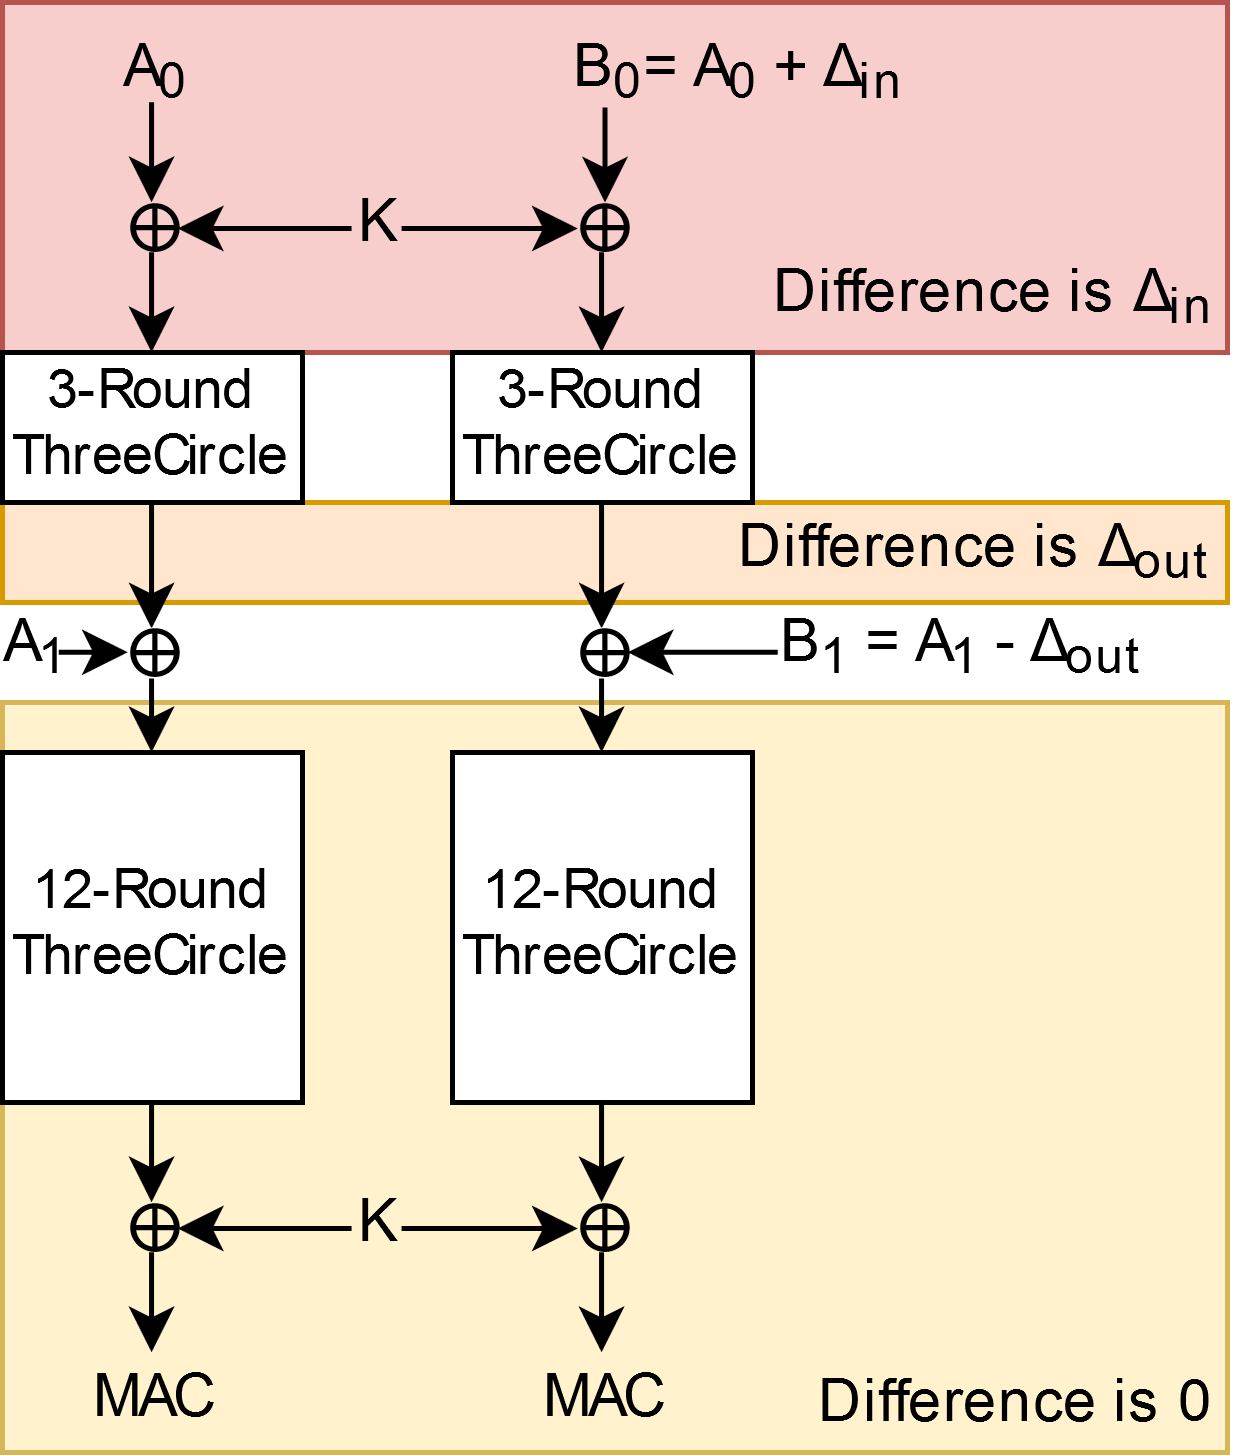
\includegraphics[scale=0.20]{imgs/Collision.png}
\caption{Finding a collision using differential $(\Delta_{in}, \Delta_{out})$.}
\label{fig:coll}
\end{figure}

\section{Finding trails / differentials}
For the attack described in previous section to work, we need a differential. This section is about finding suitable differentials.

\subsection{Difference propagation in \ThreeCircle}
In order to find differentials, it is essestial to understand how differences propage in \ThreeCircle. For each layer in the round function of \ThreeCircle, we will discuss how to affects difference propagation.

\subsubsection{Non-linear layer $\chi$}

\begin{equation}
a_y \leftarrow a_y + a_{y+1}a_{y+1} \lll 1 \text{ for all } y \text{ in parallel}
\tag{$\chi$}
\end{equation}
The non-linear layer is the only layer where branching can occur. By branching we mean: given an input difference, multiple output differences are possible.
To be precise, each active (i.e.\ non-zero) digit in the difference cause 3 equally probable branches. We call the number of active digits the weight or $w$. The number of possible branches is $3^w$. The higher the amount of branches, the lower the differential probability, and thus the lower the probability of the collision attack succeeding.

\subsubsection{Mixing layer $\theta$}
\begin{equation}
\begin{split}
&p \leftarrow a_0 + a_1 + a_2 + a_3 + a_4 \\
&e \leftarrow p \lll 12 + p \lll 17 \\
&a_y \leftarrow a_y + (e \lll y) \text{ for all } y
\end{split}
\tag{$\theta$}
\end{equation}
The mixing layer only affects the difference when there are non-zero digits in the columnwise parity of the difference. It causes diffusion which means that it causes more non-zero digits in the differential. Note that this layer is linear and does not directly cause branching, but it does so indirectly since there will be more active digits in the differential the next time $\chi$ will be performed.

\subsubsection{Transposition layer $\rho \circ \pi$}
\begin{equation}
a_y \leftarrow a_{y+1} \text{ for all } y \text{ in parallel}
\tag{$\pi$}
\end{equation}
\begin{equation}
a_y \leftarrow a_y \lll r_y \text{ for all } y \text{ with } r = (0, 2, 6, 11, 19)
\tag{$\rho$}
\end{equation}
This layer also is linear and moves the digits around. It does not cause branching, but ensures that local differences spread throughout the entire state faster.

\subsection{Manually finding 1 and 2 round trails}
Finding a low weight trail that spans 1 round is trivial. We simply take the smallest non-zero difference possible: the difference with one digit set to 1. It does not matter which digit we pick. Since we only have one active digit, the weight of the differential going into $\chi$ is 1, yielding 3 branches.
This means $DP(\Delta_{in}, \Delta_{out}) = 3^{-1} = \frac{1}{3}$. One possible differential is shown in Figure \ref{fig:1r}.
\begin{figure}
\begin{verbatim}
Input difference:
1 . . . . . . . . . . . . . . . . . . . . . . . . . . . . . . .
. . . . . . . . . . . . . . . . . . . . . . . . . . . . . . . .
. . . . . . . . . . . . . . . . . . . . . . . . . . . . . . . .
. . . . . . . . . . . . . . . . . . . . . . . . . . . . . . . .
. . . . . . . . . . . . . . . . . . . . . . . . . . . . . . . .

Output difference:
. . . . . . . . . . . . . . 1 . . . . 1 . . . . . . . . . . . .
. . . . . . . . . . . 1 . . . . 1 . . . . . . . . . . . . . . .
. . . . . . 1 . . . . 1 . . . . . . . . . . . . . . . . . . . .
1 . . . . 1 . . . . . . . . . . . . . . . . . . . . . . . . . .
. 1 . . . . . . . . . . . 1 . . . . . . . . . . . . . . 1 . . .
\end{verbatim}
\caption{Differential for 1 round of \ThreeCircle.}
\label{fig:1r}
\end{figure}

It is slightly more difficult to find one that spans two rounds.
We put two digits in the same column such that their sum is 0. This means the column-wise parity is remains 0, causing $\theta$'s' effect to be 0 as well, preventing diffision. Since the transposition layer only moves digits around, this makes it so that there are two active digits in the differential going into $\chi$ in the second round. Therefore, $DP(\Delta_{in}, \Delta_{out}) = 3^{-(2+2)} = 3^{-4} = \frac{1}{81}$. An example of this type of differential is shown in Figure \ref{fig:2r}.

\begin{figure}
\begin{verbatim}
Input difference:
2 . . . . . . . . . . . . . . . . . . . . . . . . . . . . . . .
1 . . . . . . . . . . . . . . . . . . . . . . . . . . . . . . .
. . . . . . . . . . . . . . . . . . . . . . . . . . . . . . . .
. . . . . . . . . . . . . . . . . . . . . . . . . . . . . . . .
. . . . . . . . . . . . . . . . . . . . . . . . . . . . . . . .

Output difference:
2 . . . . . . . . . . . . . 1 . . . . 1 . . . . . . . 2 . . . .
. . . . . . . . . . . 1 . . . . 1 . . . . . . . 2 . . . . 2 . .
. . . . . . 1 . . . . 1 . . . . . . . 2 . . . . 2 . . . . . . .
1 . 2 . . 1 . . . . . . . 2 . . . . 2 . . . . . . . . . . . . .
. 1 . . . . . . . 2 . . . 1 2 . . . . . . . . . . . . . 1 . . .
\end{verbatim}
\caption{Differential for 2 rounds of \ThreeCircle.}
\label{fig:2r}
\end{figure}

\section{Finding trails using evolutionary algorithms}
As we are looking for a trail that spans increasingly more rounds, reasoning about the difference propagation rapidly gets more complex as well. So complex in fact, that we could not find a good differential by hand.

Essentially, finding good trails can be seen as an optimization problem: we want to find the input difference, and according output difference that yields the highest differential probability.
A problem however is the large size of the search space: there are already 160 digits in the input difference that together can assume $3^{160}$ possible values.

We tackle this problem using a class of optimization algorithms called Evolutionary Algorithms (EAs).
Evolutionary algorithms are a type of generic population-based optimization algorithm. Evolutionary algorithms use mechanisms inspired by biological evolution, such as reproduction, mutation, recombination and selection~\cite{back1996evolutionary}. Candidate solutions play the role of individuals in a population, and the fitness function determines the quality of the solutions.

EAs often work well on NP-problems.
It is however not guaranteed to return the best solution and is based on assumptions that are not necessarily true, most notably the building block hypothesis. Roughly speaking, it hypothesizes that good solutions can be combined into a solution that is even better.

\subsection{Implementation}
EAs are actually quite simple to implement, namely as follows:
\begin{enumerate}
\item Generate the initial population of individuals randomly.
\item Evaluate the fitness of each individual.
\item Repeat until termination:
\begin{itemize}
  \item Select the best-fit individuals for reproduction.
  \item Breed new individuals through crossover and mutation.
  \item Evaluate the individual fitness of new individuals.
  \item Replace least–fit population with new individuals.
\end{itemize}
\end{enumerate}
There are many design decisions to make when implementing an EA.
There are many flavors for selection, mutation, recombination and reproduction to choose from.
But perhaps the most important one is the fitness function, since it is a single figure of merit that summerizes how close a solution is to achieving a set of aims. If chosen poorly, the algorithm will not work and will either converge on a poor solution or not at all. The fitness function should favor trails with a higher differential probability. For a solution to achieve this, the number of branches must be minimized. This means we need to minimize the number of active digits going into $\chi$.

We tried a number of variants, but what worked best for us was the sum of weights of the differential going into $\chi$ for each round. One problem is that two input values do not always follow the same trail, causing the fitness function to be noisy.

Our implementation does not implement an EA from scratch but instead uses DEAP~\cite{deap2012jmlr}, an evolutionary computation framework. We use the \texttt{eaSimple} function with a population size of 300, 50 generations, a probability of $\frac{1}{3}$ to start mutation, and subsequently a probability of $\frac{2}{5*32} = \frac{1}{80}$ for each digit to mutate into a random value.

To counteract the noisiness of the fitness function, we run it a number of times (e.g. 100 times) and then use the trail with lowest sum of weights. This works because there are many equally good trails, and for determining the fitness, we only need to hit one of the trails that have lowest weight.

Furthermore, since we emperically know that good trails tend to have many zeroes in them, we bias the digits in the randomly generated initial population towards 0.

\subsection{Results}
The EA helped us find trails that span 3 rounds that have a differential probability of $3^{16}$. This was very surprising as we anticipated that the best trail would have a differential probability of $3^{26}$. These trails are all zero except for a 2 in the second last lane with an 1 underneath it in the last lane. An example is shown in Figure \ref{fig:3r}. The existence of these trails reveals a weakness in the rotation constants of \ThreeCircle. In conclusion, it might be worth pursuing the use of evolutionary algorithms to find trails for differential cryptanalysis.
\begin{figure}
\begin{verbatim}
Input difference:
. . . . . . . . . . . . . . . . . . . . . . . . . . . . . . . .
. . . . . . . . . . . . . . . . . . . . . . . . . . . . . . . .
. . . . . . . . . . . . . . . . . . . . . . . . . . . . . . . .
. . . . . . . . . . . . . . . . . . . 2 . . . . . . . . . . . .
. . . . . . . . . . . . . . . . . . . 1 . . . . . . . . . . . .

Output difference:
1 1 . 1 2 2 . . 1 1 2 . . 2 2 2 . 1 2 . . 2 2 1 2 2 1 . . 1 2 1
2 2 2 . . 2 1 2 1 . 1 2 . . 1 . 2 . 2 2 1 2 1 1 . . 2 2 1 1 1 .
1 1 . 1 . 1 2 . . 1 2 2 2 2 2 1 2 2 1 . . 2 2 1 1 1 . 1 2 . . .
2 2 . . 2 2 . 2 2 1 . 2 1 . . 2 2 1 1 1 1 1 2 2 . 1 1 1 2 1 . 1
2 2 . . 2 1 2 2 1 2 . 2 2 . 1 1 . 1 2 2 . . 1 . 2 1 . 1 2 2 . 1
\end{verbatim}
\caption{Differential for 3 rounds of \ThreeCircle.}
\label{fig:3r}
\end{figure}

\section{The hypercube technique}
A hypercube-like structure of messages and differences can be used to enhance the collision attack.
It is not a very complicated technique, but we found that at it is very difficult to understand at first. Furthermore, it does not help that no one seems to have written a proper explanation on it yet. For that reason, we decided to document the hypercube technique very elaborately. As we will soon explain, the technique is not viable to use with \ThreeCircle, but it might be usable with other cryptographic systems. We implemented a collision attack for 2 rounds using the hypercube technique in \path{DC/hypercube.py}.

\paragraph{The naive way of finding collisions.}
Remember, to find a collision we first need a differential characteristic ($\Delta_{in}, \Delta_{out}$).
We would then generate two messages $X_0$ and $Y_0$ such that $Y_0 = X_0 + \Delta_{in}$. When put through n rounds of \ThreeCircle, we assume that the difference between the messages equals $\Delta_{out}$ i.e.\ that $\text{n-Round3C}(X_0) = \text{n-Round3C}(Y_0) + \Delta_{out}$. Then, to compensate for the difference, we would select $Y_1$ to equal $X_1 - \Delta_{out}$. After addition of the second part of the messages, the internal states are the same, which will clearly result in a collision.

\begin{figure}[ht!]
\centering
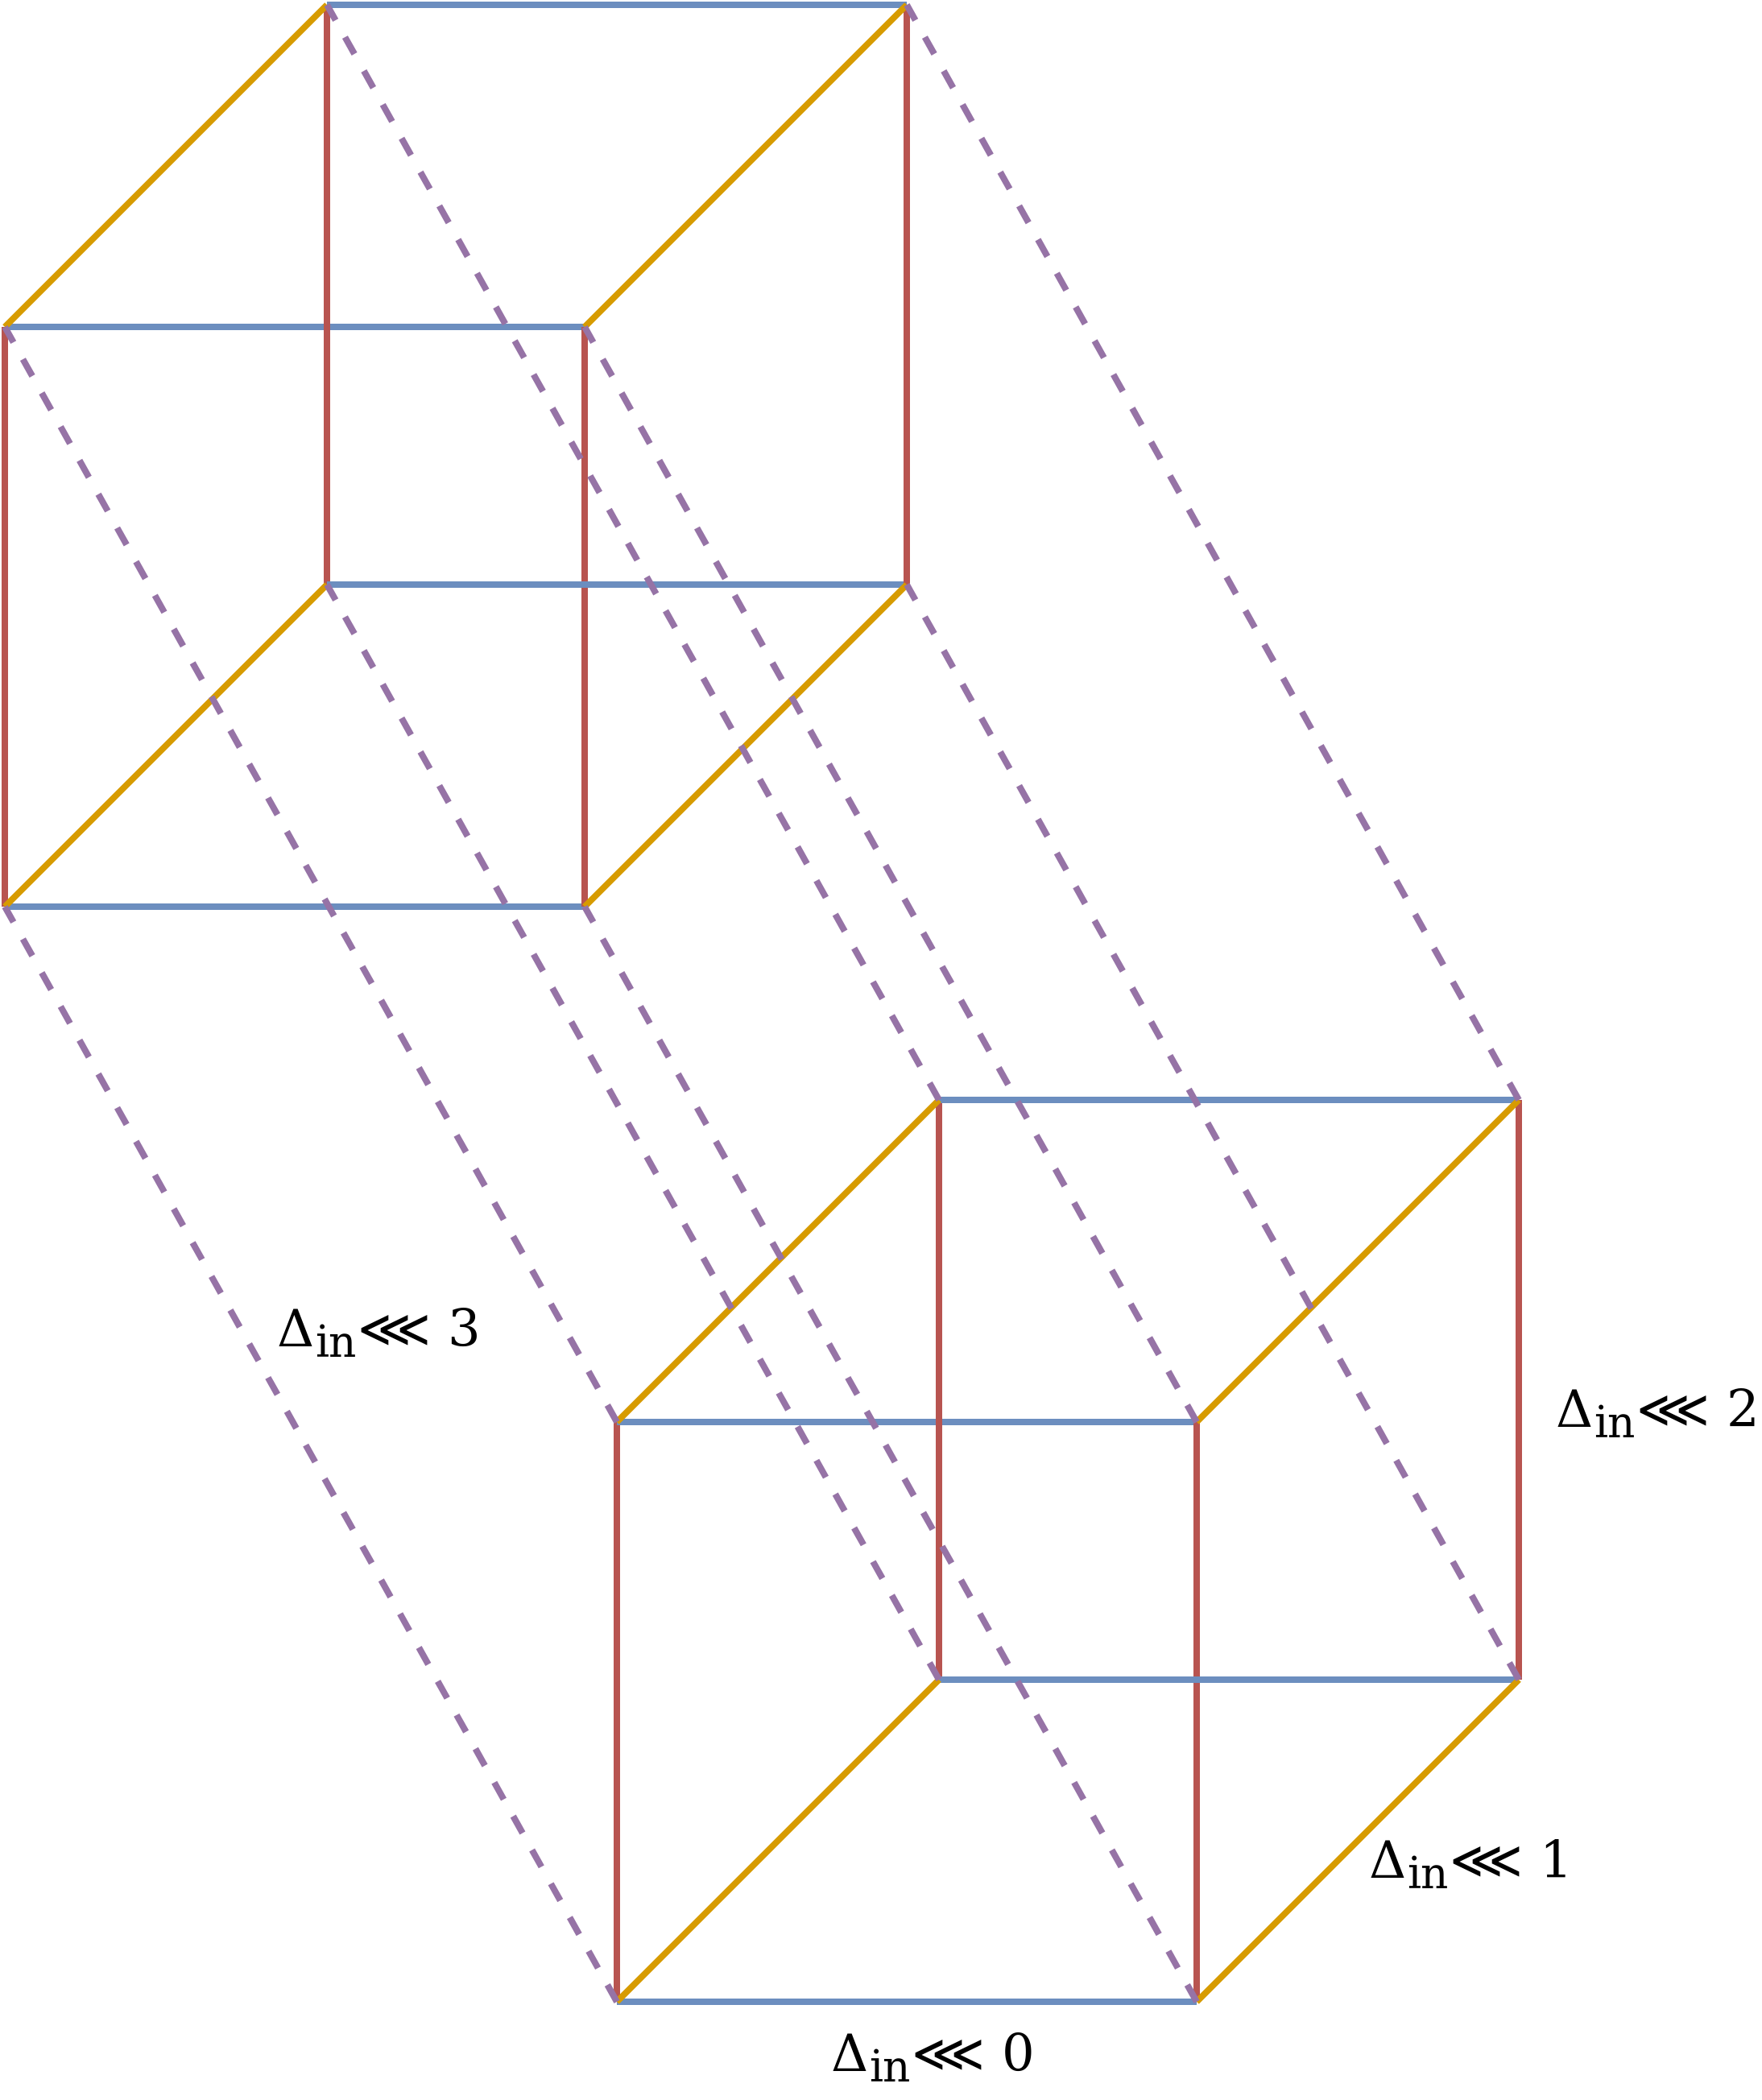
\includegraphics[scale=0.1]{imgs/hypercube.png}
\caption{4-dimensional hypercube for finding collisions.}
\label{fig:hypercube}
\end{figure}
\paragraph{Building the hypercube.}
To find collisions, we will build an n-dimensional hypercube. This structure consists of $2^n$ nodes, each of which connected to $n$ other nodes through edges. Moveover, each node represents a message input to MAC. We will choose the MACs at each node thoughtfully, such that there is an increased chance of collision between any two nodes that are directly connected through an edge.

To do this, we need one trail per dimension of the hypercube. We initialize the root node of the hypercube with MAC$(M^0_0 || M^0_1)$ for arbitrary $M^0$.

In the case of 2-round \ThreeCircle, we only need 1 trail, which we can shift to obtain new trails. We can do so utilizing a symmetry property, namely that if the input difference is shifted, the output difference is shifted in the same manner. In general one would need a list, of trails, and then use the one at index $i$ instead of shifting the first one by $i$.

The remainder of the nodes on the hypercube is now determined and defined as:
\begin{align}
\begin{split}
&MAC(M^{(a_{n-1},\dots, a_0)}_0 || M^{(a_{n-1}, \dots, a_0)}_1) \text{ such that }\\
&\forall i: a_i \in \{0, 1\} \text{ and } \\
&M^{(a_{n-1},\dots, a_0)}_0 = M^0_0 + \sum_i a_i(\Delta_{in} \lll i) \text{ and }\\
&M^{(a_{n-1},\dots, a_0)}_1 = M^0_1 - \sum_i a_i(\Delta_{out} \lll i)
\end{split}
\end{align}
Figure \ref{fig:hypercube} shows an example of a 4-dimensional hypercube.
The color of each edge shows which dimension it traverses, from which we can derive which differential must be used.

\paragraph{Why it should work.} Without loss of generality, take two adjacent nodes i.e.\ two nodes that are connected through an edge:
$MAC(M^x_0||M^x_1$) and\\$MAC(M^y_0||M^y_1)$.
We convert x and y into a binary representation which gives us \\$MAC(M^{(x_{n-1},\dots, x_0)}_0 || M^{(x_{n-1},\dots, x_0)}_1)$
and $MAC(M^{(y_{n-1},\dots, y_0)}_0 || M^{(y_{n-1},\dots, y_0)}_1)$.
Since the nodes are connected, we know that $x_i$ and $y_i$ are the same for all but one $i$.
Again, without loss of generality, assume that $x_j$ is 0 whereas $y_j$ is 1. The means that we can write $M^x_0 + (\Delta_{in} \lll j) = M^y_0$ and $M^x_1 - (\Delta_{out} \lll j) = M^y_1$.
As you can see, these two nodes can be used to find a collision through ``the naive way of finding collisions'' as the differences of the first part equal $(\Delta_{in} \lll j)$, and the second part compensates for the expected $(\Delta_{out} \lll j)$ in output difference after putting the first parts through $n$ rounds of \ThreeCircle. 

Note that the situation described above applies to each pair of nodes that is connected through an edge, and as each node takes part in not 1 but $n$ such pairs, the chances of finding a collision are greatly improved.

\paragraph{Why it does not work in this specific case.}
We implemented the hypercube strategy and verified that the hypercube was built as intended,.
We performed some experiments and discovered that it would either find no collisions or large amount of them. As it turns out, there is a large amount of interdependence between the input values - 2 or 3 rounds of \ThreeCircle simply does not scramble the outputs sufficiently. The result is that we either get no collisions at all or get a collision on every edge that crosses a certain dimension. This means that the hypercube in this case is not a viable strategy.

\chapter{Key recovery using collisions}
After finding a collision it is possible to recover part of the key. In this chapter we will show how that is done and discuss the implementation of such an attack against the MAC scheme using 2 rounds of \ThreeCircle as round-reduced transformation.

\section{Key recovery}
To recover the key, we will apply our knowledge of two colliding input values and the trail they followed to the non-linear layer of the first round.

We denote the first parts of the two colliding messages with $a$ and $a^*$. Furthermore we have a trail and a key $K$. We denote the differential going into $\chi$ as $a' = a^* - a$ and the difference after $\chi$ as $b' = b^* - b$. We know that the values going into $\chi$ are $a + K$ and $a^* + K$. $\chi$ for the first and second message are $b_i = a_i + a_j^2$ and $b_i^* = a_i^* + {a_j^*}^2$ respectively.
\begin{equation}
\begin{split}
b_i' &= b_i^* - b_i \\
&= a_i^* + {a_j^*}^2 - (a_i + a_j^2) \\
&= (a_i^* - a_i) + ({a_j^*}^2 - a_j^2) \\
&= (a_i^* - a_i) + (a_j + a_j')^2 - a_j^2 \\
&= a_i + a_j^2 + 2a_ja_j' + a_j' - a_j^2 \\
&= a_i  + 2a_ja_j' + a_j' \\
a_j &= \frac{b_i' - a_i' -a_j'^2}{2aj'}
\end{split}
\label{eq:recover}
\end{equation}
We now know the actual value $a_j$ that is going into $\chi$. Furthermore, we know that that value is the addition of the message and the key. We know this value and we know the message, so with a simply subtraction, we can recover the key.

For this to work $2a_j'$ must be invertible in $\GF(3)$. This is the case when it is different from 0. In other words, the digit at position $j$ in the differential must be non-zero in order for us to be able to recover the digit of the key at position $j$. Therefore in order to recover the entire key, we need a series of differentials such that the non-zero digits in the input differences together cover all 160 digits of the state.

One can easily generate a set of differentials with non-zero digits that cover the entire state for 1 and 2 rounds of \ThreeCircle by making use of symmetry and shifting both the input and output difference. We do not have such symmetry when there are 3 rounds. Furthermore, non-zero digits in the input difference of the efficient trails only cover the bottom two lanes. Therefore one would need other trails to recover the other digits. These trails will probably have a much smaller differential probability.

\section{Implementation}
The attack consists of two parts:
\begin{itemize} 
\item Collect a number of trails of collisions such that all digits of the key can be recovered;
\item Apply Equation \ref{eq:recover} to the collected trails and recover the key.
\end{itemize}

\noindent\path{DC/trail_collector.py} collects trails for inputs that collide over 2 rounds of \ThreeCircle. Utilizing the symmetry property it finds good input/output pairs that cover the entire state, allowing for recovery of the entire key. For each pair it searches for collisions in the usual manner, that is, picking random messages $X$ and computing according message $Y$ until they collide. Eventually, it exports the found trails in JSON format.\\

\noindent\path{DC/key_recovery.py} imports the trails and recovers one digit of the key per trail using Equation \ref{eq:recover}. To do so, it must reconstruct the difference directly after the non-linear transform in the first round. To this end, it applies the inverse round and subsequently the inverse $\lambda$ function to the output difference recorded in the trail. Eventually, as a test, it compares the extracted key to the actual key.

\bibliography{bibliography.bib}
\end{document}